%% Section that includes the experiments performed.

This section describes the accomplished experiments that prove how the developed system fulfills SKA's requirements for the PPS distribution system. The first experiment is a general characterization of the developed platform. The second one, tests the equipment in a realistic network topology to evaluate the performance in a possible deployment. The last experiments evaluates the influence of some typical events, such as traffic, temperature fluctuation or \textcolor{blue}{something else} in a network deployment using the WR-ZEN.

Performance of the new WR platform is measured using multiple equipment, and obtained results have been compared to WRS's performance because of it's electronic design is considered as reference for WR technology. The list of the equipment and materials used for the experiments is the following:

\begin{itemize}
    \item Two White Rabbit Switches to simulate a typical WR network. All of them have hardware version 3.4 and 5.0 of firmware.
    \item A White Rabbit ZEN Time Provider (WR-ZEN TP) to test the performance of the new developed platform as node of a WR network. The firmware version is 1.2.
    \item Phase noise plots, ADEV, TDEV and TIE measures have been taken using a Symmetricom 3120A.
    \item PPS stability tests have been measured with a Keysight 53230A Timer.
    \item The 3120A needs an external stable clock reference. That reference is also needed as input for the WR equipment when Grand Master mode is set. A Morion MV89 Oven Controlled Crystal Oscillator (OCXO) has been used as clock reference for the experiments.
    \item Multiple components for the setup of the equipment:
    \begin{itemize}
        \item Small form-factor pluggable transceptors (SFPs) to stablish the link between WR devices.  \textcolor{blue}{\textit{TODO:} Completar cuando se hayan usado}
        \item Optical fiber links. \textcolor{blue}{\textit{TODO:} Completar con las fibras que se hayan usado}
        \item \textcolor{blue}{\textit{TODO:} Something else?}
    \end{itemize}
    \item \textcolor{blue}{\textit{TODO:} Completar conforme se hagan medidas}
\end{itemize}

\subsection{Characterization of the WR-ZEN platform}
\label{subsec: charact_zen}

% Aquí las pruebas típicas de caracterización

The new components included in the clocking's scheme of the WR-ZEN (fig. ?), described in subsection \ref{subsec:hardware}, offer a performance improvement respect to previous WR designs, such as the WRS. 

\missingfigure{Esquema de las medidas realizadas}

The following experiments evaluate phase noise performance of the frequency transfer in WR at different scenarios: a) Grand Master mode, to evaluate how the WR-ZEN syntonizes to an external reference clock. b) Master mode, that reflects the characteristics of the new internal XO of the WR-ZEN. c) Slave mode, to see the behavior of the new design as slave node of the network. Different configurations are depicted in fig. ?? to allow the reproduction of the different experiments of this paper.

\missingfigure{testing schemas}

The Free running mode (FR) is not affected by the WR's logic, it is mostly influenced by noise of the crystal oscillator (XO). A master node is placed at top of a timing network hierarchy, and unlike a Grand Master node, it is not locked to any external reference. So that, a master node with an improved stability will benefit the performance of all the downlink devices connected to it.

Picture \ref{fig:zen_vs_wrs} shows an high jitter accumulation in low frequencies for the WRS (orange curve). Integrating noise from 1Hz to 10 Hz, we see a difference of 60.1 ps of RMS jitter between WRS and WR-ZEN. Other results can be checked in table \ref{tab:pn_results}. It is worthy to remark difference between sine wave output and TTL output in the WR-ZEN board. As detailed in fig. ?? \textit{(clock schema)} there are two 10 Mhz clock outputs in the WR-ZEN. One comes directly from the AD9516-4 PLL, the sine wave output. The other, comes from FPGA logic but it is latched using a clock signal from the LMK03806 PLL. It would be foreseeable to expect an higher jitter in the signal from the FPGA, but thanks to the low noise profile of the LMK PLL we can remove much of the jitter of that signal and decrease the floor noise of it.

\begin{figure}[t]
	\centering
	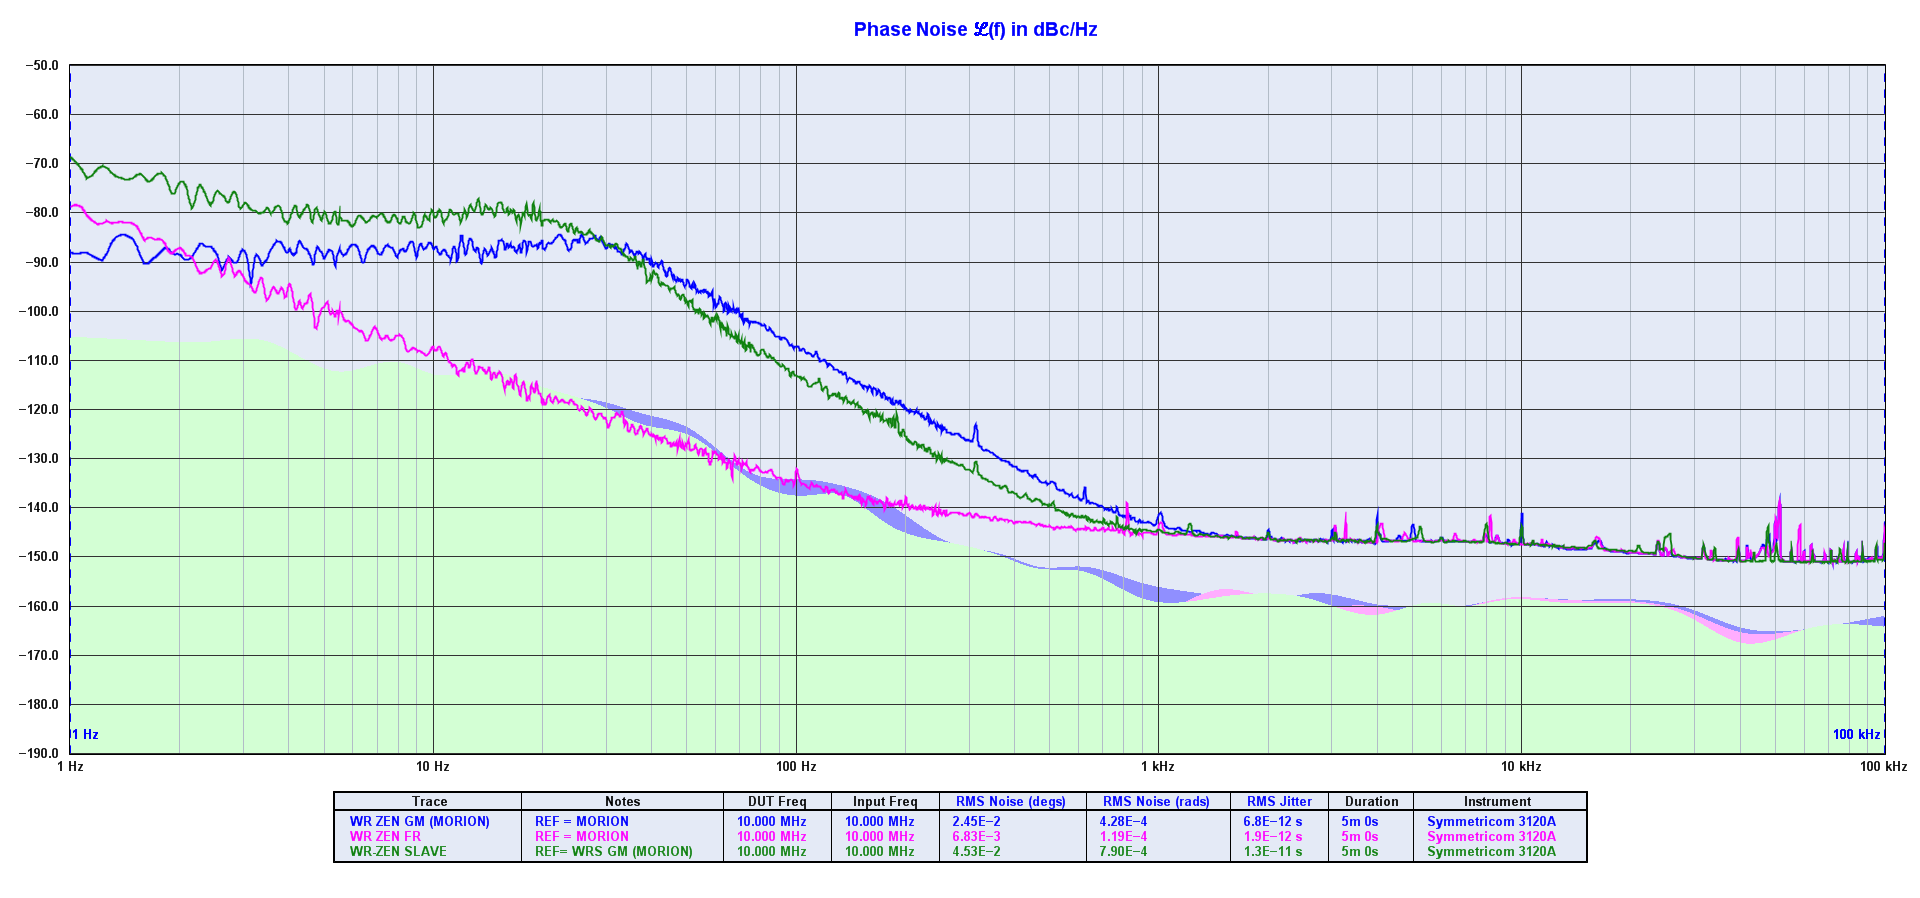
\includegraphics[width=0.8\textwidth]{../measures/img/zen_all}
	\caption[Phase noise plot of the WR-ZEN]{The figure shows the Phase noise plot for the WR-ZEN in the Grand Master, Free Running and Slave modes. Sine wave output is compared to CMOS output.}
	\label{fig:zen_pn_all}
\end{figure}

\begin{figure}[t]
	\centering
	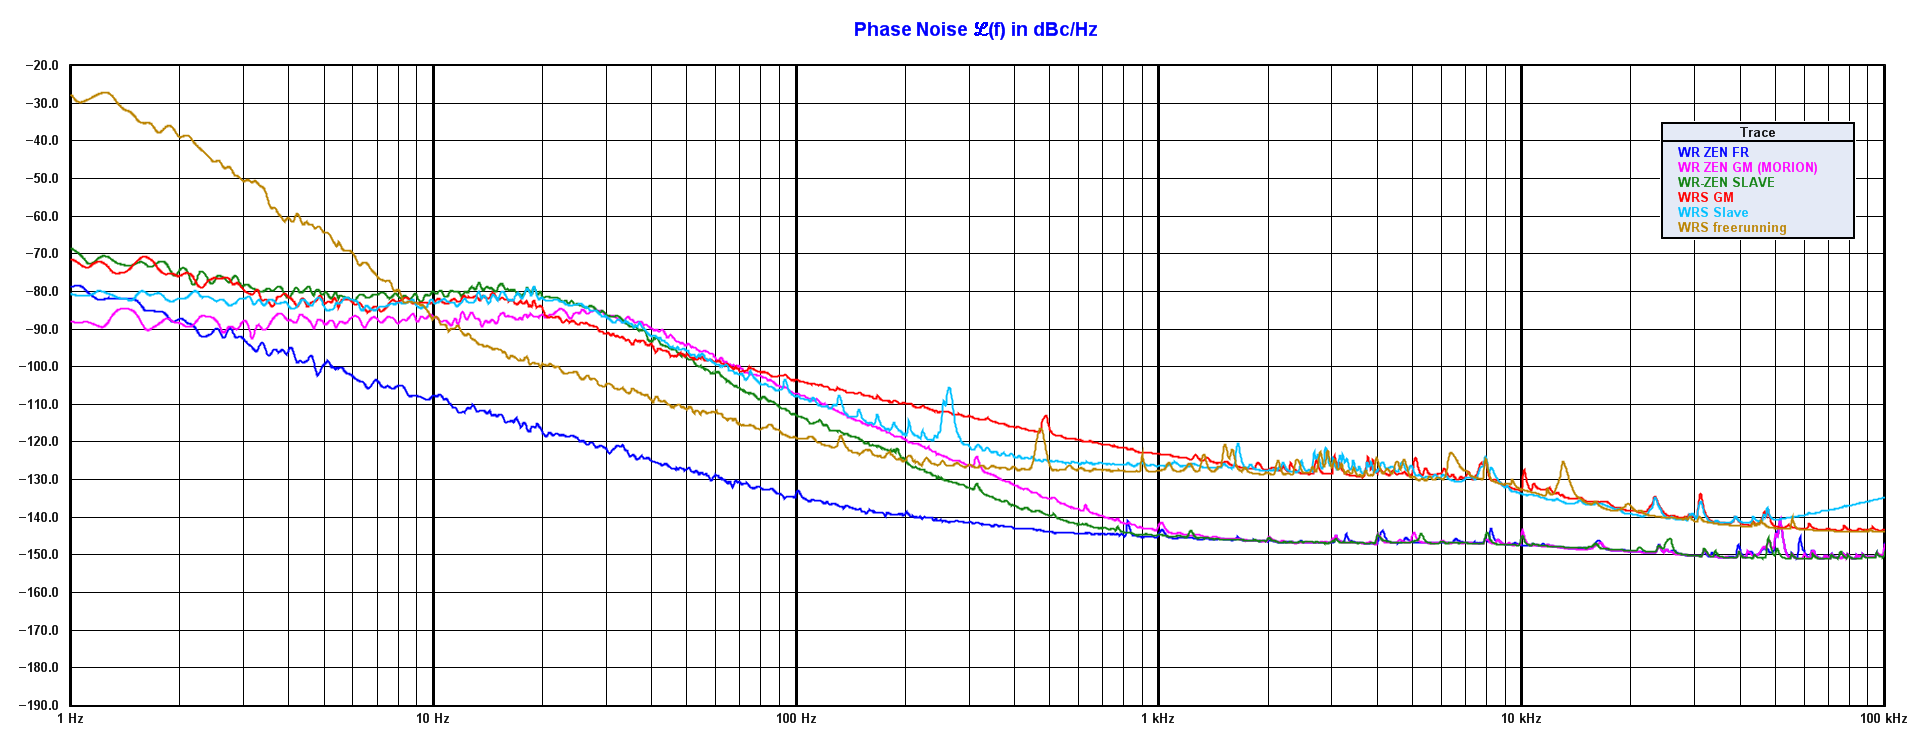
\includegraphics[width=0.8\textwidth]{../measures/img/zen_vs_wrs}
    \caption[Phase noise plot of the WR-ZEN vs WRS]{The figure includes the same phase noise measures for the WRS. In this plot, only the CMOS outputs appear because the WRS doesn't have sine wave output signals.}
    \label{fig:zen_vs_wrs}
\end{figure}

It is also relevant testing the performance of the system when locking to an external reference in Grand master mode because the board is intended to be used as Time Provider. Additive noise of the WR-ZEN will be propagated downstream, decreasing the quality of the Grand master's reference clock. It's very important that the system adds low noise in order to not degrade the quality of the external reference clock.

Results included in table \ref{tab:pn_results} and ploted in figure \ref{fig:zen_vs_wrs} unveil a jitter reduction in the WR-ZEN compared to the WRS of 2.1 ps of RMS jitter integrated from 1Hz to 100kHz. This is a relevant because jitter in the slave nodes will benefit from a noise reduction in the Grand Master node.    
    
 \begin{table*}\centering
     \ra{0.8}
     \begin{tabular}{@{} rcccc@{}}%\toprule
         & \multicolumn{4}{c}{\bfseries{RMS jitter (ps)}} \\
         \cmidrule(l){2-5}
         & 1Hz-10Hz & 10Hz-1kHz & 1kHz-100kHz  & 1Hz-100kHz \\ \midrule
         \textbf{Free running}\\
         \small{WRS (CMOS)}             & 62  & 1.7  & 1.1  & 62  \\
         \small{WR-ZEN (\textit{sine})} & 2.1 & 0.24 & 1.4  & 2.5 \\
         \small{WR-ZEN (\textit{CMOS})} & 1.9 & 0.21 & 0.26 & 1.9 \\
         \cmidrule(l){2-5}
         
         \textbf{Grand Master}\\
         \small{WRS (CMOS)}             & 7.3 & 6.7 & 1.1 & 9.9\\
         \small{WR-ZEN (\textit{CMOS})} & 2.8 & 6.2 & 0.26 & 6.8\\
         \cmidrule(l){2-5}
         
         \textbf{Slave node}\\
         \small{WRS (CMOS)}             & 4.9 & 8.2 & 1.2  & 9.7\\
         \small{WR-ZEN (\textit{CMOS})} & 8.5 & 9.3 & 0.24 & 13\\
         
         \bottomrule
        \end{tabular}
        \caption{Phase Noise results extracted from plots in figure \ref{fig:zen_pn_all} and \ref{fig:zen_vs_wrs}.}
        \label{tab:pn_results}
\end{table*}

The slave mode results show that WR-ZEN performs slightly worse than WRS. Noise between 1 Hz and 20 Hz increases the RMS Jitter of the WR-ZEN in ?? \textit{sacar de los datos en crudo!!}. The observed difference could be caused by a bad adjustment of some of the internal parameters of the control loop for the slave mode. This will be treated in future work because the scope of this contribution is characterize the initial design of the WR-ZEN.

\subsection{Network experiment} %% Buscar un nombre mejor
\label{subsec: net_exp}

The next experiment covers the analysis of timing distribution over a WR network formed by a WRS in the top of the hierarchy locked to an external reference (Grand Master), an intermediate WRS and a final node, the WR-ZEN. We planned to reproduce an example of time distribution for the SKA facilities where it won't be there so many hops between the clock reference and end nodes. \ftglnote{Esto me suena de que era así pero no recuerdo y estoy vago para comprobarlo. Si es mentira eliminarlo!} For the experiment we kept devices under laboratory conditions: temperature and humidity controlled, absence of external noise sources and so on. For a more realistic tests under changing conditions, see results from ?? (\textit{meter ref a paul aquí???}).

\missingfigure{diagrama de la configuración del experimento}

Some time-domain results are presented in table ?? and fig. ?? because of the importance of that kind of measures for time distribution networks. This time, we have take the PPS outputs from WRS and WR-ZEN and we have performed some long time measurements and plotted them with a Time Deviation (TDEV) analysis.

\missingfigure{plot TDEV}

Hablar de los resultados cuando los calcule del todo.

\missingfigure{tabla MTIE}

\subsection{Traffic influence on synchronization accuracy}

% Posible experimento metiendo tráfico a la cadena anterior

\subsection{Redundancy}

% Este no me queda muy claro, cuando toque se verá

\subsection{Thermal characterization...}

% Aquí irían el de la cámara térmica, mover las fibras para simular viento y
% chorradas por el estilo

 
